\sect{2 \quad Matched images, endpoints and communication}
\begin{center}\small
\begin{tabular}{@{}lrrll@{}}\toprule
Site & Calibration pool & Evaluation & Evaluation order & Positive reference\\\midrule
Cornell FGVC7 \cite{thapa} &450&1,353&5 fixed hash orders&Any labelled disease\\
Kashmir \cite{yatoo} &256&384&5 fixed hash orders&Any labelled disease\\
Latvia \cite{kodors} &590&579&Nine later dates, EXIF&Visible apple scab\\\bottomrule
\end{tabular}
\end{center}
For each site, a content-identity order defines 20 nested draws with 16, 32 and 128 calibration candidates. The camera can retain candidate images or their addresses in a calibration reservoir. Their labels are held until purchase. Latvia's calibration pool comes from the five early capture days. Across the calibration and evaluation splits we found no equal file hashes. The minimum cross-split 64-bit perceptual Hamming distances were 6, 10 and 12. The 579 Latvian evaluation records contain 578 distinct exact images. Cornell and Kashmir lack usable timestamps for these streams. Their orders are replay assumptions.

Three pipelines share calibration identities, evaluation frames and the same frozen PlantDoc-balanced DINOv2 cloud expert \cite{dino}. The released V2 model has a 160-pixel input and a 0.30 disease cutoff \cite{agri}. The CPU V2-grid pipeline preserves that cutoff and applies the release's tensor scales and S3 rounding rule to the V2 graph. The MobileNetV4-Conv-Small pipeline uses ImageNet pretraining, a PlantDoc-trained source head and a 0.50 cutoff \cite{vfour}. Its architecture, training sources and operating point jointly define this second pipeline. Both V2 and V4 use the same 1,280-dimensional packed-head interface. The V2-grid pipeline is a host approximation whose embedded fixture differs from the actual device result.

\subt{Reference labels and paired comparisons}
We use $\mathrm{BA}=(\mathrm{sensitivity}+\mathrm{specificity})/2$ and retain the original binary error counts. An already labelled pilot, an available but unlabelled candidate, and an evaluation image play different roles. The selection rule can receive newly purchased labels for the first two actions and receives the cloud's output on evaluation images only if they are sent. An independent evaluator opens evaluation labels after the predicted decisions exist. Every result at a given site, pipeline, arrival order and budget uses the same evaluation identities and JPEG lengths. Fixed caps on annotation allow methods to spend different amounts. The exact-label comparison in Section 4 holds the acquired identities and setup cost equal.

\newpage
\sect{3 \quad Pay for the pilot, then choose whether to update}
\begin{center}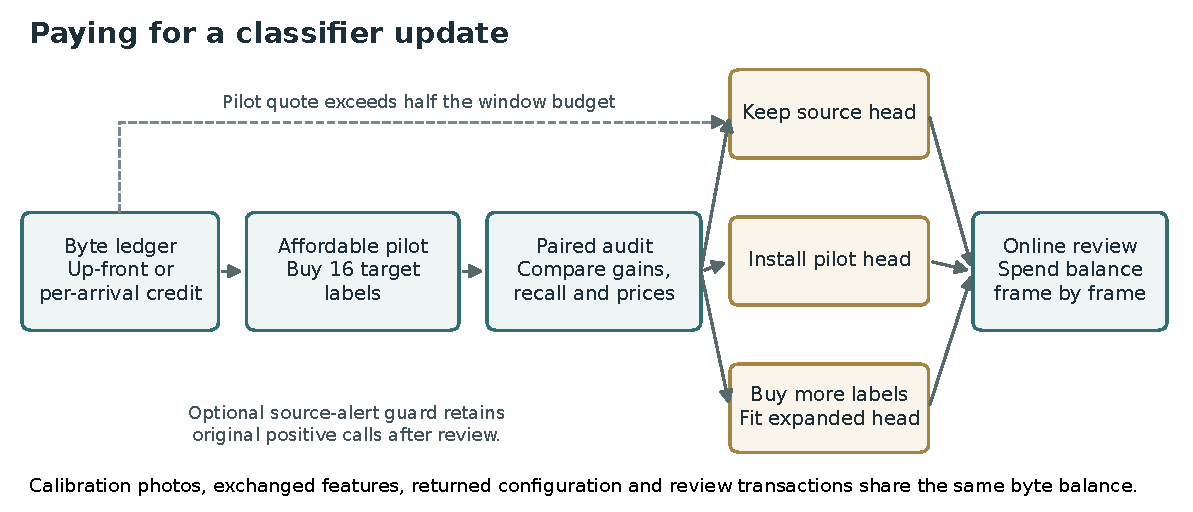
\includegraphics[width=.97\linewidth]{figures/purchase_flow.pdf}\end{center}
\note{Figure 1. Calibration and inference share a single ledger. In the earned condition funds accumulate from zero. A single compressed evaluation frame can be queried at each arrival.}

The nominal full rate is 6,800 application bytes per arrival. We test 680, 1,700 and 3,400 bytes per arrival. The prepaid grant supplies the entire window allowance upfront. The earned grant starts at zero and releases bytes as frames arrive, without borrowing. All purchase, installation and inference costs are charged. A human label requires the actual quality-75 JPEG, an image envelope, a 1,293-byte activation record, a four-byte source score, and a 12-byte receipt. A purchase includes a 32-byte request and eight-byte action packet. Each returned head costs 1,294 bytes, and learned routers add their serialized weights. A review consumes its actual 224-pixel JPEG plus 20 bytes. Service is instantaneous in these replays.

Before opening any target label, the controller compares the 16-image pilot quote with half the planned allowance. If it buys the pilot, it compares the existing camera and a candidate head on held-out folds of those photos. It prices the remote queries each action could afford using past prices and scores, estimates improvement with a shrinkage penalty for small class counts, and requires no observed sensitivity loss on the pilot. A nested learning-curve comparison can authorize expansion. Training uses only purchased labels. The synthetic stream scores future evaluations only after the policy has chosen its purchase, and it releases the chosen action only when the corresponding bytes can be debited. Local source calls continue while accumulating credit. The stream uses the preceding 64 local scores, an online estimate of JPEG cost, and a shared percentile gate. The comparison with the calibrated fixed EdgeBoost cutoff preserves its threshold semantics.
